\pdfoutput=1
\documentclass{JINST}
\let\ifpdf\relax

\usepackage{epsfig}
\usepackage{subfigure}
\usepackage{wrapfig}
\usepackage{multirow}

\title{Parallel Computing and the Search for Jets and Black Holes at the LHC}

\author{V. Halyo\thanks{Corresponding Author}, A. Hunt, P. Jindal, P. LeGresley, P. Lujan \\
\llap Princeton University, Princeton, NJ, USA \\
E-mail: \email{vhalyo@gmail.com}}

\abstract{Abstract goes here...

}
\keywords{ATLAS; CMS; Level-1 trigger; HLT; Tracker system; Jets; Black holes}

\begin{document}

\section{Introduction} 

Data analysis at the LHC requires approaches to processing that are effective at finding the underlying physics phenomena while still being cost efficient.  Using computing technologies derived from consumer products results in lower hardware acquisition costs because many of the research, development, and manufacturing costs are amortized over much larger volumes.  These consumer products are increasingly mobile devices such as phones, tables, and notebook computers so there is significant interest in energy efficiency to maximize battery life.  This focus on energy efficiency also the potential to benefit more traditional areas of computing and data analysis by reducing operating costs such as electrical power and cooling.

Leveraging processors derived from consumer products helps minimize costs associated with purchasing and operating large compute installations such as required for the LHC, but there is also a software aspect that needs to be considered.  Moore's Law continues to yield ever more powerful processors but the architecture of processors has changed significantly over the past decade.  For many years CPUs were able to run the exact same software faster and faster with each new generation of processor.  This changed in the early 2000s as Intel and AMD shifted focus to multicore processors featuring at first two cores, but with some newer processors featuring as many as 16 cores.

Parallel processors, in the form of multicore CPUs and more recently highly programmable Graphics Processing Units (GPUs), may require a significant rethink of algorithms and their implementations.  At the same time the High Energy Physics (HEP) community is at a crossroads with tentative confirmation of the Higgs particle completing the search for particles predicted by the Standard Model.  The search for physics beyond the Standard Model will require development of advanced algorithms for detecting rare new physics phenomena, and these new algorithms will need to be designed and implemented based on knowledge of the current state and likely future directions for processor architecture.

\section{Physics Motivation}





\section{Parallel Processor Architecture}

When discussing computer processors it is common to bring up Moore's Law.  However, it is important to recognize what Moore's Law actually represents.  Moore's Law is an empirical observation made by Intel co-founder Gordon Moore in the 1960s that it was economically feasible to double the number of transistors on a single integrated circuit every 24 months.  So although modern usage tends to associate Moore's Law with processor performance it is first and foremost about manufacturing technology and the ability to fabricate ever smaller transistors.

In terms of performance, one of the most obvious benefits of smaller transistors is the ability to run processors at faster clock rates.  Over the course of a few years processor clock speeds jumped from tens of MHz to GHz speeds.  However, manufacturers were not able to fully decrease operating voltages in a corresponding way and this led to increases in power density and the inability to dissipate that power out of such a small area.  For the first time processors had become power limited.

It is fairly clear how a faster clock speed yields a faster processor.  What is a little less obvious is how more transistors can make a single core processor faster even at fixed clock speeds.  Additional transistors available at each generation of Moore's Law allowed hardware designers to implement Instruction Level Parallelism (ILP).  Instead of the processor executing one operation per clock cycle (an arithmetic operation, a load from memory, a store back to memory, etc.) multiple instructions are executed in parallel.  For example, a load from memory is issued for a future arithmetic operation, an arithmetic operation is performed, and a store back to memory of a previous arithmetic operation is issued.  This hardware based parallelism in x86 processors is determined dynamically as the program is executing and allows arbitrary single-threaded software to run faster by exploiting parallelism within the instruction stream.

With ever more transistors, the implementation of ILP and the associated techniques of instruction pipelining, out-of-order execution, speculative execution, and hardware branch predictors helped consume many of the additional transistors made available through Moore's Law.  But in addition to ILP, the growing gap between the performance of the processors running at GHz speeds and the off chip memory systems necessitated adding a complicated cache hierarchy to modern processors.

Also mention SIMD / SSE??

While compute performance may increase around 60\% per year in accordance with Moore's Law, memory performance increases approximately 10\% year.  If left unchecked this would have resulted in processors that were theoretically very computationally powerful but would be limited in practical performance because of the constant need to wait on memory traffic.  To address this modern processors have a complicated cache hierarchy not only for data, but also for instructions, and even for translating virtual memory addresses to physical memory addresses in the form of Translation Lookaside Buffers (TLB).  Additional logic in the form of hardware prefetchers observe memory access patterns in real time and attempt to prefetch into the caches instructions and data that are likely to be needed in the future.  The disparity between processor and memory performance is so bad that the vast majority of the processor is devoted not to computation but to data handling.  As shown in Figure~\ref{fig:core_i7_die} the L3 cache plus the memory controller and other I/O portions of the chip easily represent around 50\% of the area.  Within each of the cores are the L1 and L2 caches, plus all of the logic associated with ILP.  The actual chip area devoted to computation is remarkably small.

\begin{figure}[!Hhtb]
\begin{center}
	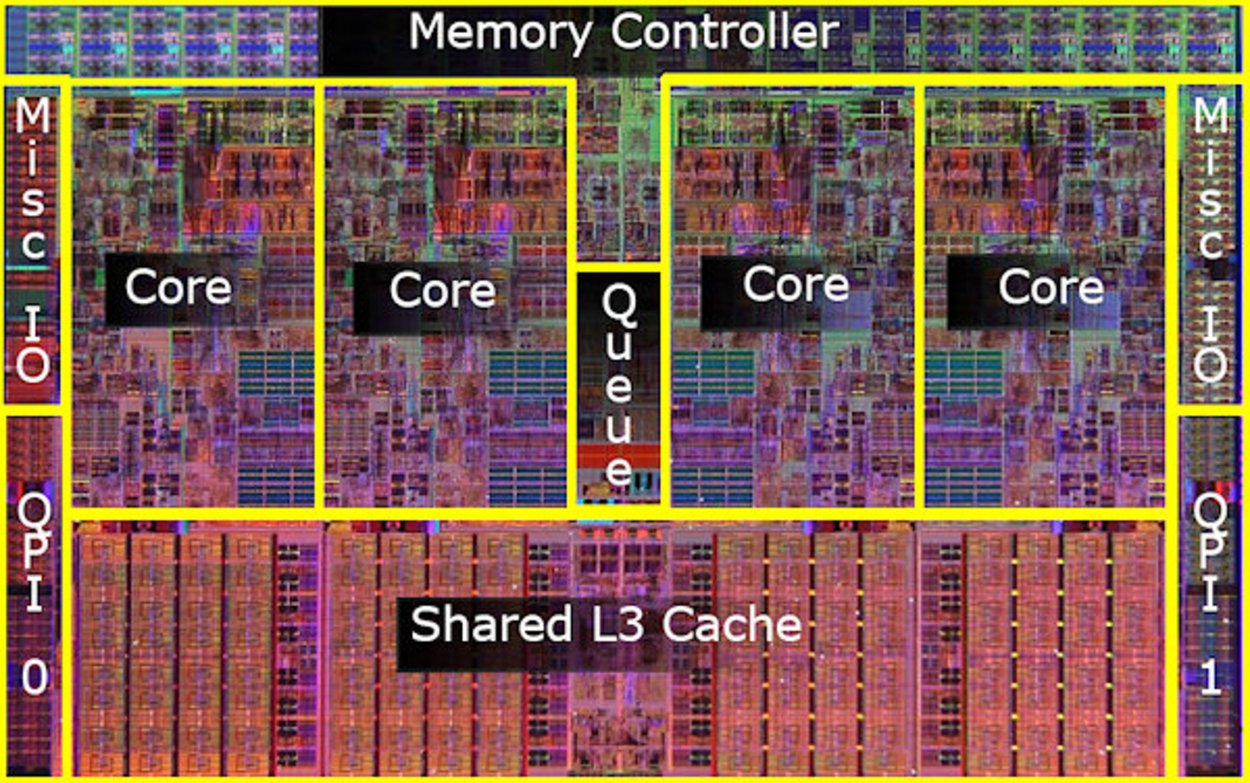
\includegraphics[width=1.0\textwidth]{figs/Core_i7_die.pdf}
	\caption{Intel Core i7 die showing major components of the processor (image from Intel). \label{fig:core_i7_die}}
\end{center}
\end{figure}

Nonetheless, these improvements in hardware had the advantage of using existing software and simply running it faster.  However, there are limits to what the hardware can do to automatically extract ILP and predict the memory access pattern of arbitrary applications.  Deep instruction pipelines, which in some processors exceeded 30 stages, have issues with hazards that would affect the correctness of results if not correctly handled by the processor, stalls due to unavailability of inputs, and mispredicted branching behavior.  At some point this complexity reaches a level of diminishing returns where the hardware complexity (and hence cost) outweigh the benefits.

With faster clock speeds not feasible and ILP also reaching its limits, hardware designers in the early 2000s turned to multicore to utilize all of those additional transistors available to them from Moore's Law.  As shown in Figure~\ref{fig:core_i7_die}, the hardware designers design a core, plus the hardware logic to link them together, and can then place as many cores on a single chip as current manufacturing technology allows.



GPUs

Intel Xeon Phi


\section{Hough Transform Algorithm}

Review algorithm and what we've done already

\section{Jet and Black Hole Detection}

New stuff ....

\section{Results}

Figures, tables, etc.

\section{Summary}

\end{document}